\documentclass[]{standalone}
\usepackage{amsmath,amssymb}
%matrix
\newcommand{\mt}[1]{\ensuremath{\mathbf{#1}}}
%vector
\newcommand{\vc}[1]{\ensuremath{\boldsymbol{#1}}}
%set
\newcommand{\st}[1]{\ensuremath{\mathcal{#1}}}
%time index
\newcommand{\tm}[1]{\ensuremath{\sp{(#1)}}}


%x
\newcommand{\x}[0]{\ensuremath{\vc{x}}}
%s
\newcommand{\s}[0]{\ensuremath{\vc{s}}}
%W
\newcommand{\W}[0]{\ensuremath{\mt{W}}}



\usepackage{pgf}
\usepackage{tikz}
\usetikzlibrary{arrows,automata,matrix}
\usepackage[latin1]{inputenc}
\begin{document}
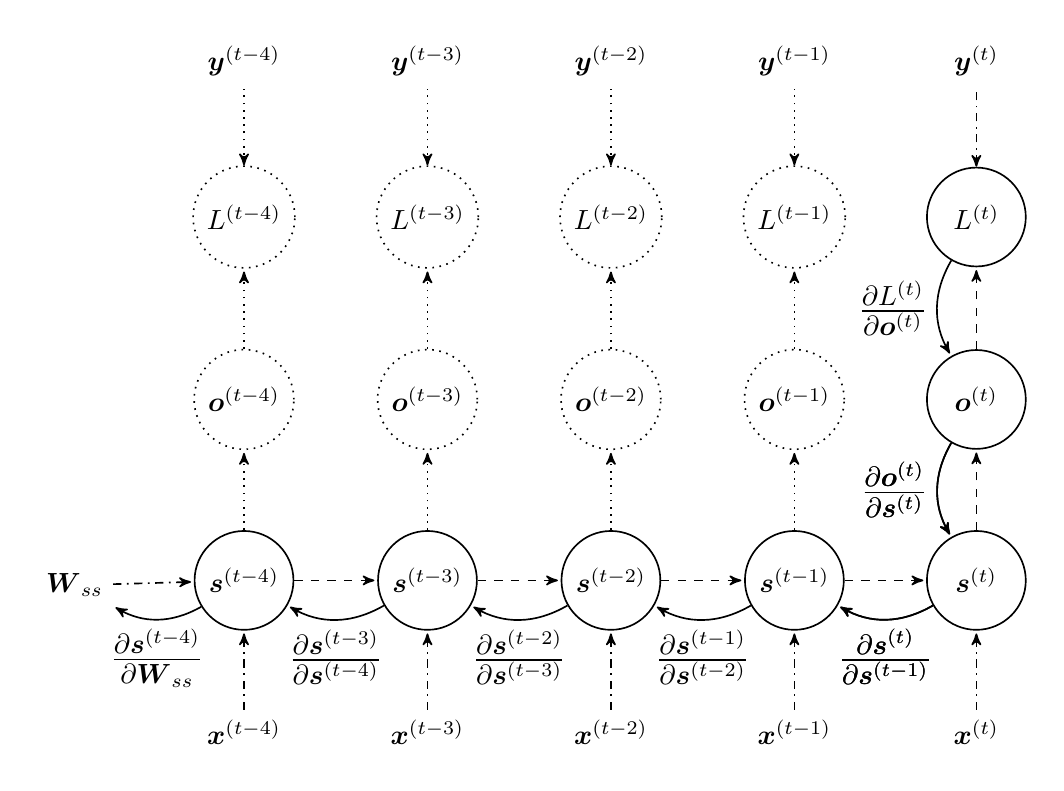
\begin{tikzpicture}[->,>=stealth'
	,shorten >=1pt
	,auto
	,node distance=2.8cm,
              semithick]
  \tikzstyle{every state}
  =[minimum size={10pt+width("$x^{(t-1)}$")}
  ,dotted]

  \matrix (m) [matrix of nodes
  ,row sep=.4in,column sep=.4in] {
    % 5 ys
    &
    \node[](y4) {$\vc{y}\tm{t-4}$};      &
    \node[](y3) {$\vc{y}\tm{t-3}$};      &
    \node[](y2) {$\vc{y}\tm{t-2}$};      &
    \node[](y1) {$\vc{y}\tm{t-1}$};      &
    \node[](y0) {$\vc{y}\tm{t}$};        \\
    % 5 Ls
    &
    \node[state](L4) {$L\tm{t-4}$}; &
    \node[state](L3) {$L\tm{t-3}$}; &
    \node[state](L2) {$L\tm{t-2}$}; &
    \node[state](L1) {$L\tm{t-1}$}; &
    \node[state,solid](L0) {$L\tm{t}$};
    \\
    % 5 os
    &
    \node[state](o4) {$\vc{o}\tm{t-4}$}; &
    \node[state](o3) {$\vc{o}\tm{t-3}$}; &
    \node[state](o2) {$\vc{o}\tm{t-2}$}; &
    \node[state](o1) {$\vc{o}\tm{t-1}$}; &
    \node[state,solid](o0) {$\vc{o}\tm{t}$};   \\
    % 5 ss + W
    \node[](Wss)       {$\vc{W}_{ss}$};         &
    \node[state,solid](s4) {$\vc{s}\tm{t-4}$}; &
    \node[state,solid](s3) {$\vc{s}\tm{t-3}$}; &
    \node[state,solid](s2) {$\vc{s}\tm{t-2}$}; &
    \node[state,solid](s1) {$\vc{s}\tm{t-1}$}; &
    \node[state,solid](s0) {$\vc{s}\tm{t}$};   \\
    % 5 xs
    &
    \node[](x4) {$\vc{x}\tm{t-4}$};      &
    \node[](x3) {$\vc{x}\tm{t-3}$};      &
    \node[](x2) {$\vc{x}\tm{t-2}$};      &
    \node[](x1) {$\vc{x}\tm{t-1}$};      &
    \node[](x0) {$\vc{x}\tm{t}$};      \\
  };


  % verticals
  %-4
  \path[->,dashdotted] (x4) edge node {} (s4);
  \path[->,dotted] (s4) edge node {} (o4);
  \path[->,dotted] (o4) edge node {} (L4);
  \path[<-,dotted] (L4) edge node {} (y4);
  %-3
  \path[->,dashdotted] (x3) edge node {} (s3);
  \path[->,dotted] (s3) edge node {} (o3);
  \path[->,dotted] (o3) edge node {} (L3);
  \path[<-,dotted] (L3) edge node {} (y3);
  %-2
  \path[->,dashdotted] (x2) edge node {} (s2);
  \path[->,dotted] (s2) edge node {} (o2);
  \path[->,dotted] (o2) edge node {} (L2);
  \path[<-,dotted] (L2) edge node {} (y2);
  %-1
  \path[->,dashdotted] (x1) edge node {} (s1);
  \path[->,dotted] (s1) edge node {} (o1);
  \path[->,dotted] (o1) edge node {} (L1);
  \path[<-,dotted] (L1) edge node {} (y1);
  %-0
  \path[->,dashdotted] (x0) edge node {} (s0);
  \path[->,dashed] (s0) edge node {} (o0);
  \path[->,dashed] (o0) edge node {} (L0);
  \path[<-,dashdotted] (L0) edge node {} (y0);
  % horizontals
  %-3
  \path[->,dashdotted] (Wss)  edge node {} (s4);
  \path[->,dashed] (s4) edge node {} (s3);
  \path[->,dashed] (s3) edge node {} (s2);
  \path[->,dashed] (s2) edge node {} (s1);
  \path[->,dashed] (s1) edge node {} (s0);


\tikzset{every edge/.append style={font=\Large}}

  %diffs from dL/dW

  \path[bend right]
  (L0) 
  edge node[left] {
    $\frac{\partial{L}\tm{t}}
    {\partial{\vc{o}}\tm{t}}$}
  (o0) ;

  \path[bend right]
  (o0) 
  edge node[left] {
    $\frac{\partial{\vc{o}\tm{t}}}
    {\partial{\vc{s}\tm{t}}}$}
  (s0) ;

  \path[bend right]
  (o0) 
  edge node[left] {
    $\frac{\partial{\vc{o}\tm{t}}}
    {\partial{\vc{s}\tm{t}}}$}
  (s0) ;

  \path[bend left]
  (s0) 
  edge node[below] {
    $\frac{\partial{\vc{s}\tm{t}}}
    {\partial{\vc{s}\tm{t-1}}}$}
  (s1) ;

  \path[bend left]
  (s1) 
  edge node[below] {
    $\frac{\partial{\vc{s}\tm{t-1}}}
    {\partial{\vc{s}\tm{t-2}}}$}
  (s2) ;

  \path[bend left]
  (s2) 
  edge node[below] {
    $\frac{\partial{\vc{s}\tm{t-2}}}
    {\partial{\vc{s}\tm{t-3}}}$}
  (s3) ;

  \path[bend left]
  (s3) 
  edge node[below] {
    $\frac{\partial{\vc{s}\tm{t-3}}}
    {\partial{\vc{s}\tm{t-4}}}$}
  (s4) ;

  \path[bend left]
  (s0) 
  edge node[below] {
    $\frac{\partial{\vc{s}\tm{t}}}
    {\partial{\vc{s}\tm{t-1}}}$}
  (s1) ;

  \path[bend left]
  (s4) 
  edge node[below] {
    $\frac{\partial{\vc{s}\tm{t-4}}}
    {\partial{\vc{W}_{ss}}}$}
  (Wss) ;


%oh ok. input W-> 
%get 'back' an 'update' for W thru ds/dW
  
\end{tikzpicture}

\end{document}